\section{The Joint Multiple Multilevel Estimation Framework}
\label{sec:sec2}

\subsection{Formulation}
Suppose there are $K$ independent datasets, each pertaining to an $M$-layered Gaussian Graphical Model (GGM). The $k^{\Th}$ model has the following structure:

\vspace{1em}
\begin{tabular}{ll}
{\it Layer 1}- &
%
$\BD_1^k = (D_{1 1}^k, \ldots, D^k_{1 p_1}) \sim
\cN (0, \Sigma_1^k); \quad k \in \cI_K,$\\
{\it Layer $m$} $(1< m \leq M)$-  &
%
$ \BD_m^k = \BD_{m-1}^k \bfB_m^k + \BE_m^k$, with $\bfB_m^k \in \BM(p_{m-1}, p_m) $\\
& and $\BE_m^k = (E_{m 1}^k, \ldots, E^k_{m p_m}) \sim
\cN (0, \Sigma_m^k); \quad k \in \cI_K $.\\
\end{tabular}
\vspace{1em}

We assume known structured sparsity patterns, denoted by $\cG_m$ and $\cH_m$, for the parameters of interest in the above model, i.e. the precision matrices $\Omega_m^k := (\Sigma_m^k)^{-1}$ and the regression coefficient matrices $\bfB_m^k$, respectively. These patterns provide information on horizontal dependencies across $k$ for the corresponding parameters, and our goal is to leverage them to estimate the full hierarchical structure of the network -specifically to obtain the undirected edges for the nodes inside a single layer, and the directed edges between two successive layers through jointly estimating $\{ \Omega_m^k \}$ and $\{ \bfB_m^k \}$.

Consider now a two-layer model, which is a special case of the above model with $M=2$:
%
\begin{eqnarray}
\BX^k = (X^k_1, \ldots, X^k_p)^T \sim \cN (0, \Sigma^k_{x});\\
\BY^k = \BX^k \bfB^k + \BE^k; \quad \BE^k = (E^k_1, \ldots, E^k_p)^T \sim \cN (0, \Sigma^k_{y});\\
\bfB^k \in \BM(p,q), \quad \Omega^k_{x} = (\Sigma^k_{x})^{-1}; \quad \Omega^k_y = (\Sigma^k_{y})^{-1};
\end{eqnarray}
%
wherein we want to estimate $\{ (\Omega^k_{x}, \Omega^k_{y}, \bfB^k); k \in \cI_K \}$ from data $\cZ^k = \{ (\bfY^k, \bfX^k); \bfY^k \in \BM(n,q), \bfX^k \in \BM(n,p), k \in \cI_K\}$ in presence of known grouping structures $\cG_x, \cG_y, \cH$ respectively and assuming $n_k = n$ for all $k \in \cI_K$ for simplicity. We focus the theoretical discussion in the remainder of the paper on jointly estimating $\Omega_{y}:= \{ \Omega_{y}^k \}$ and $\cB := \{ \bfB^k \}$. This is because for $M>2$, within-layer undirected edges of any $m{\Th}$ layer $(m>1)$ and between-layer directed edges from the $(m-1){\Th}$ layer to the $m{\Th}$ layer can be estimated from the corresponding data matrices in a similar fashion (see details in \citet{LinEtal16}). On the other hand, parameters in the very first layer are analogous to $\Omega_{x} := \{ \Omega_{x}^k \}$, and can be estimated from $\{ \bfX^k\}$ using any method for joint estimation of multiple graphical models (e.g. \citet{GuoEtal11, MaMichailidis15}). This provides all building blocks for recovering the full hierarchical structure of our $M$-layered multiple GGMs.

%Setting $M=1$ reduces the above model to joint estimation of GGMs with structured sparsity \citep{MaMichailidis15}, while setting $K=1$ reduces the model to a multi-layer GGM, which can be estimated by breaking it down to successive two-layer models and then minimizing a penalized conditional log-likelihood function \citep{LinEtal16}.

\subsection{Algorithm}
\label{sec:algosection}

\begin{figure}
\centering
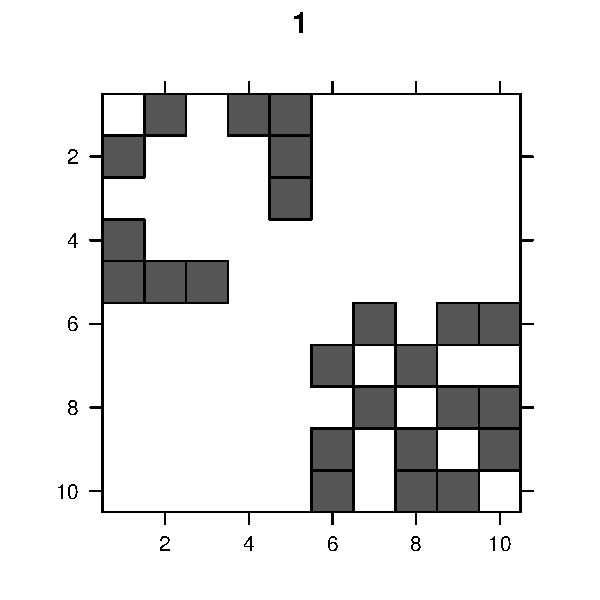
\includegraphics[width=.23\textwidth]{adj1}
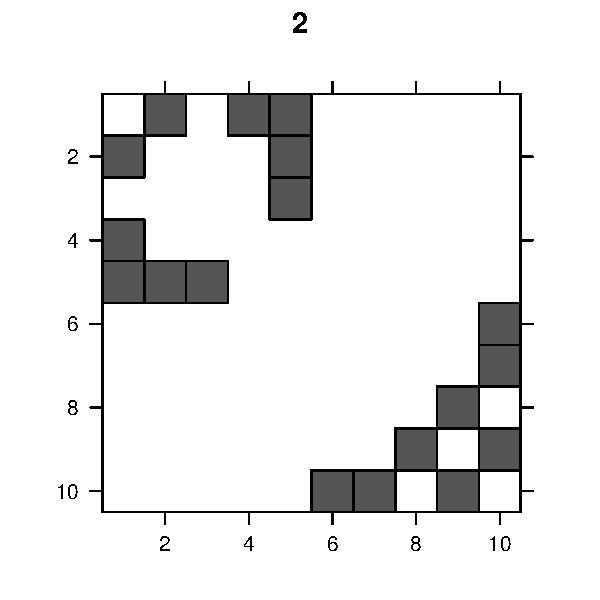
\includegraphics[width=.23\textwidth]{adj2}
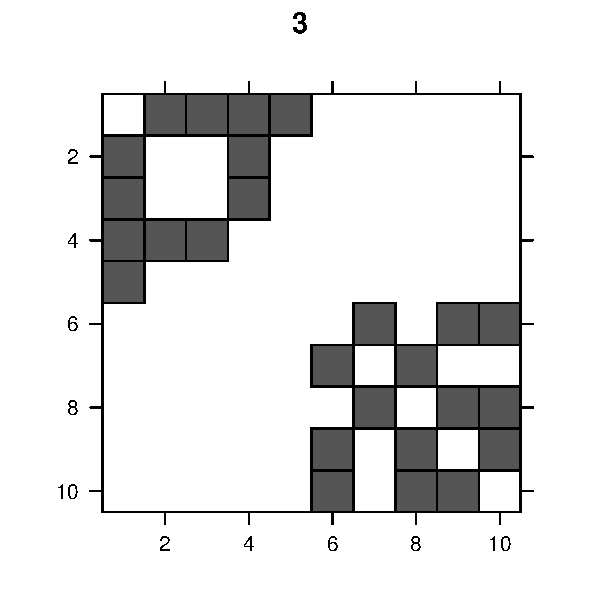
\includegraphics[width=.23\textwidth]{adj3}
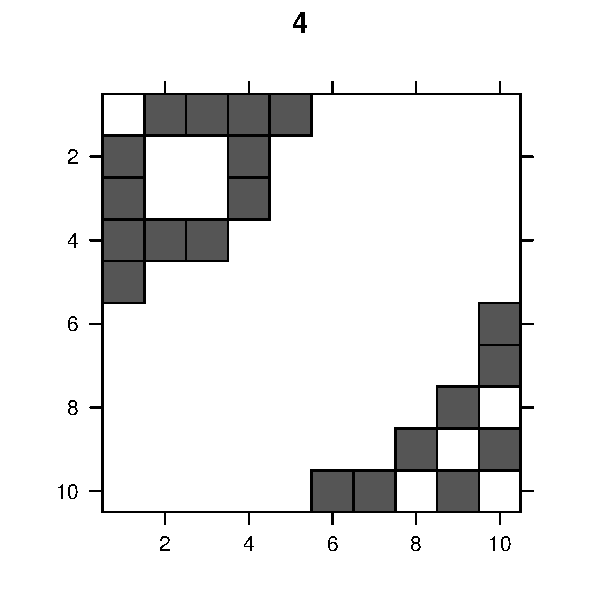
\includegraphics[width=.23\textwidth]{adj4}
\caption{Shared sparsity patterns for four $10 \times 10$ precision matrices. for elements $\cG_{x,ii'}$ in the upper $5 \times 5$ block, matrices (1,2) and (3,4) have the same non-zero support, i.e. $\cG_{x,ii'} = \{ (1,2),(3,4)\}$. On the other hand, when $i,i'$ are in the lower block, $\cG_{x,ii'} = \{ (1,3),(2,4)\}$}
\label{fig:jsem-exmaple}
\end{figure}


We assume an element-wise group sparsity pattern over $k$ for the precision matrices $\Omega_x^k$:
%
\[
\cG_x = \{ \cG_x^{ii'}: i \neq i'; i, i' \in \cI_p \},
\]
%
where each $\cG_x^{ii'}$ is a partition of $\cI_K$, and consists of index groups $g$ such that $g \subseteq \cI_K, \cup_{g \in \cG_x^{ii'}} g = \cI_K$. First introduced in \citet{MaMichailidis15}, this formulation helps incorporate group structures that are common across some of the precision matrices being modeled. Figure~\ref{fig:jsem-exmaple} illustrates this through a small example. Subsequently, we use the Joint Structural Estimation Method (JSEM) \citep{MaMichailidis15} to estimate $\Omega_x$, which first uses the group structure given by $\cG_x$ in penalized nodewise regressions \citep{MeisenBuhlmann06} to obtain neighborhood coefficients $\zeta_i = (\bfzeta_i^1, \ldots, \bfzeta_i^K)$ of each variable $X_i, i \in \cI_p$, then fits a maximum likelihood model over the combined support sets to obtain sparse estimates of the precision matrices:
%
\begin{align}\label{eqn:jsem-model}
\widehat \zeta_i &= \argmin_{\zeta_i} \left\{
\frac{1}{n} \sum_{k=1}^K \| \bfX_i^k - \bfX_{-i}^k \bfzeta_i^k \|^2 +
\sum_{i' \leq i} \sum_{g \in \cG_x^{ii'}} \eta_n \| \bfzeta_{ii'}^{[g]} \| \right\}, \notag\\
\widehat E_x^k &= \{(i,i'): 1 \leq i < i' \leq p, \hat \zeta_{ii'}^k \neq 0 \text{ OR } \hat \zeta_{i'i}^k \neq 0 \}, \notag\\
\widehat \Omega_x^k &= \argmin_{\Omega_x^k \in \BS_+ (\hat E_x^k)}
\left\{ \Tr (\widehat \bfS_x^k \Omega_x^k ) - \log \det (\Omega_x^k) \right\}.
\end{align}
%
where $\widehat \bfS_x^k := (\bfX^k)^T \bfX^k/n$, $\eta_n$ is a tuning parameter, and $\BS_+ (\hat E_x^k)$ is the set of positive-definite matrices that have non-zero supports restricted to $\hat E_x^k$.

For the precision matrices $\Omega_y^k$, we assume an element-wise sparsity pattern $\cG_y$ defined in a similar manner as $\cG_x$. The sparsity structure $\cH$ for $\cB$ is more general, each group $h \in \cH$ being defined as:
%
$$
h = \{ (\cS_p, \cS_q, \cS_K): \cS_p \subseteq \cI_p, \cS_q \subseteq \cI_q, \cS_K \subseteq \cI_K \}
; \quad \bigcup_{h \in \cH} h = \cI_p \times \cI_q \times \cI_K.
$$
%
In other words, any arbitrary partition of $\cI_p \times \cI_q \times \cI_K$ can be specified as the sparsity pattern of $\cB$.

Denote the neighborhood coefficients of the $j^{\Th}$ variable in the lower layer by $\bftheta_j^k$, and $\Theta_j := (\bftheta_j^1, \ldots, \bftheta_j^K), \Theta = \{ \Theta_j \}$. We obtain sparse estimates of $\cB, \Theta$, and subsequently $\Omega_y$, by solving the following group-penalized least square minimization problem that has the tuning parameters $\gamma_n$ and $\lambda_n$ and then refitting:
%
\begin{align}
\{ \widehat \cB, \widehat \Theta \} &= 
\argmin_{\cB, \Theta} \left\{ \frac{1}{n} \sum_{j=1}^q \sum_{k=1}^K \| \bfY^k_j - (\bfY_{-j}^k - \bfX^k \bfB_{-j}^k) \bftheta_j^k - \bfX^k \bfB_j^k \|^2 \right. \notag\\
& \left. + \sum_{j \neq j'} \sum_{g \in \cG_y^{jj'}} \gamma_n \| \bftheta_{jj'}^{[g]} \| + \sum_{h \in \cH} \lambda_n \| \bfB^{[h]} \| \right\}, \label{eqn:jmmle-objfun}\\
\widehat E_y^k &= \{(j,j'): 1 \leq j < j' \leq q, \hat \theta_{jj'}^k \neq 0 \text{ OR } \hat \theta_{j'j}^k \neq 0 \}, \notag\\
\widehat \Omega_y^k &= \argmin_{\Omega_y^k \in \BS_+ (\hat E_y^k)}
\left\{ \Tr (\widehat \bfS_y^k \Omega_y^k ) - \log \det (\Omega_y^k) \right\}. \label{eqn:omega-y-calc}
\end{align}
%&= \min \left\{ f ( \cY, \cX, \cB, \Theta) + P (\Theta) + Q (\cB) \right\} 
%
The outcome of a node in the lower layer is thus modeled using all other nodes in that layer using the neighborhood coefficients $\widehat \bfB_j^k$, {\it and} nodes in the immediate upper layer using the regression coefficients $\widehat \bftheta_j^k$.

\begin{Remark}
Common sparsity structures across the same layer are incorporated into the regression by the group penalties over the element-wise groups $\bftheta_{jj'}^{[g]}$, while sparsity pattern overlaps across the different regression matrices $\bfB^k$ are handled by the group penalties over $\bfB^{[h]}$, which denote the collection of elements in $\cB$ that are in $h$. Other kinds of structural assumptions on $\cB$ or $\Theta$ can be handled within the above structure by swapping out the group norms in favor of other appropriate norm-based penalties.
\end{Remark}

\begin{Remark}
Group sparsity assumptions are not necessary for the JMMLE framework: rather in a practical situation they help leverage additional information regarding interaction of features in and between the layers, {\it as and when that information is available}. In the vertical direction of the model, i.e. given a fixed $k$, a framework agnostic of any structural dependency assumptions amounts to element-wise groups in $\bfB^k$ and $\Omega_y^k$. In JMMLE, this occurs by construction for $\Theta$, and since $\cH$ consists of all possible partitions of $\cI_p \times \cI_q \times \cI_K$, it covers the case of element-wise groups as well. On the other hand, the absence of any horizontal (i.e. across $k$) dependency simply decomposes the problems \eqref{eqn:jmmle-objfun} and \eqref{eqn:omega-y-calc} into $K$ independent sub-problems that can be solved separately either by setting $K=1$ in our framework or by using existing methods, such as \citet{LinEtal16}.
\end{Remark}

\subsubsection{Alternating Block Algorithm}
The objective function in \eqref{eqn:jmmle-objfun} is bi-convex, i.e. convex in $\cB$ for fixed $\Theta$, and vice-versa, but not jointly convex in $\{ \cB, \Theta \}$. Consequently, we use an alternating iterative algorithm to solve for $\{ \cB, \Theta \}$ that minimizes \eqref{eqn:jmmle-objfun} by iteratively cycling between $\cB$ and $\Theta$, i.e. holding one set of parameters fixed and solving for the other, then alternating until convergence.

Choice of initial values plays a crucial role in the performance of this algorithm as discussed in detail in
\citet{LinEtal16}. 
% Following the analysis of \citet{LinEtal16}, who proposed an estimation framework for the special case of our multi-level structure for $K=1$ based on a similar algorithm, we choose the initial values $\{ \bfB^{k (0)} \}$ by first selecting a support set for the $j^{\Th}$ column, say $\tilde \cS_j^k$, as the support of the debiased lasso estimate of \citet{JavanmardMontanari14}, then fitting a Lasso regression model with small penalty value $\lambda_n^0$:
%
%\begin{align}\label{eqn:init-B}
%\widehat \bfB_j^{k (0)} = \argmin_{\supp(\bfB_j^k) \subseteq \tilde \cS_j^k} \|\bfY_j^k - \bfX^k \bfB_j^k \|^2 + \lambda_n^0 \| \bfB_j^k \|_1
%\end{align}
%
We choose the initial values $\{ \widehat \bfB^{k (0)} \}$ by fitting separate lasso regression models for each $j$ and $k$:
%
\begin{align}\label{eqn:init-B}
\widehat \bfB_j^{k (0)} = \argmin_{\bfB_j^k \in \BR^p} \|\bfY_j^k - \bfX^k \bfB_j^k \|^2 + \lambda_n \| \bfB_j^k \|_1; \quad
j \in \cI_q, k \in \cI_K.
\end{align}
%

We obtain initial estimates of $ \Theta_j, j \in \cI_q$ by performing group-penalized nodewise regression on the residuals $\widehat \bfE^{k (0)} := \bfY^k - \bfX^k \widehat \bfB_j^{k (0)}$:
%
\begin{align}\label{eqn:init-Theta}
\widehat \Theta_j^{(0)} = \argmin_{\Theta_j} \frac{1}{n} \sum_{k=1}^K \|
\widehat \bfE_j^{k (0)} - \widehat \bfE_{-j}^{k (0)} \bftheta_j^k \|^2
+ \gamma_n \sum_{j \neq j'} \sum_{g \in \cG_y^{jj'}} \| \bftheta_{jj'}^{[g]} \|.
\end{align}

The steps of our full estimation procedure, coined as the {\it Joint Multiple Multi-Layer Estimation} (JMMLE) method, are summarized in Algorithm \ref{algo:jmmle-algo}.

\begin{Algorithm}
(The JMMLE Algorithm)
\label{algo:jmmle-algo}

\noindent 1. Initialize $\widehat \cB$ using \eqref{eqn:init-B}.

\noindent 2. Initialize $\widehat \Theta$ using \eqref{eqn:init-Theta}.

\noindent 3. Update $\widehat \cB$ as:
%
\begin{align}\label{eqn:update-B}
\widehat \cB^{(t+1)} &= \argmin_{\substack{\bfB^k \in \BM(p,q)\\k \in \cI_K}} \left\{ \frac{1}{n} \sum_{j=1}^q \sum_{k=1}^K \| \bfY^k_j - (\bfY_{-j}^k - \bfX^k \bfB_{-j}^k) \widehat \bftheta_j^{k (t)} - \bfX^k \bfB_j^{k } \|^2
+ \lambda_n \sum_{h \in \cH} \| \bfB^{[h]} \| \right\}
\end{align}

\noindent 4. Obtain $\widehat \bfE^{k (t+1)} := \bfY^k - \bfX^k \bfB_j^{k (t)}, k \in \cI_K$. Update $\widehat \Theta$ as:
%
\begin{align}\label{eqn:update-Theta}
\widehat \Theta_j^{(t+1)} = \argmin_{\Theta_j \in \BM(q-1, K)}
\left\{ \frac{1}{n} \sum_{k=1}^K
\| \widehat \bfE_j^{k (t+1)} - \widehat \bfE_{-j}^{k (t+1)} \bftheta_j^k \|^2
+ \gamma_n \sum_{j \neq j'} \sum_{g \in \cG_y^{jj'}} \| \bftheta_{jj'}^{[g]} \| \right\}
\end{align}

\noindent 5. Continue till convergence.

\noindent 6. Calculate $\widehat \Omega_y^k, k \in \cI_K$ using \eqref{eqn:omega-y-calc}.
\end{Algorithm}

\subsubsection{Tuning parameter selection}
A number of methods have been proposed in the literature to select regularization tuning parameters in $\ell_1$-penalized problems. Some approaches rely on traditional criteria like cross-validation, Akaike Information Criterion (AIC)~\citep{DanaherEtal14} or the Bayesian Information Criterion (BIC)~\citep{LinEtal16,MaMichailidis15}. A number of studies have proposed their modifications for the case when feature dimensions increase with sample size \citep{GaoEtal12,KimKwonChoi12}.

As a demonstration, to select the tuning parameter $\lambda_n$ we use the High-dimensional BIC (HBIC, \citet{KimKwonChoi12, WangKimLi13}), and for selecting $\gamma_n$ in the node-wise regression step in the JSEM model \eqref{eqn:jsem-model}, stick to the use of BIC as done by \citet{MaMichailidis15}. Unlike BIC, the penalty term in HBIC scales with the parameter dimensions. As a result, the tuning parameter selected as the minimizer of HBIC asymptotically identifies the oracle estimator in ultra-high dimensional penalized problems \citep{FanTang13, WangKimLi13}. In our case, we train multiple JMMLE models using Algorithm \ref{algo:jmmle-algo} over a finite set of values $\lambda_n \in \cD_n$, and calculate their HBIC:
%
\begin{align*}
\text{HBIC} (\lambda_n; \Theta) &=
\frac{1}{n} \sum_{j=1}^q \sum_{k=1}^K \| \bfY^k_j - (\bfY_{-j}^k - \bfX^k \widehat \bfB_{-j,\lambda_n}^k ) \bftheta_j^{k } - \bfX^k \widehat \bfB_{j,\lambda_n}^k \|^2 +\\
& \log (\log n) \frac{\log (pq)}{n} \sum_{k=1}^K
\left( \| \bfB^k \|_0 + | \widehat E_{y, \gamma_n^* (\lambda_n)}^k| \right).
\end{align*}
%
Following this, we choose the optimal $\lambda_n$ as the empirical minimizer of HBIC over $\cD_n$: $
\lambda^* = \argmin_{\lambda_n \in \cD_n} \text{HBIC} (\lambda, \widehat \Theta_{\gamma_n^*(\lambda_n)})
$.

The step for updating $\Theta$, i.e. \eqref{eqn:update-Theta}, in our JMMLE algorithm is analogous to the JSEM method \citet{MaMichailidis15}, hence we use BIC to select the penalty parameter $\gamma_n$. In our setting the BIC for a given $\gamma_n$ and fixed $\cB$ is given by:
%
\begin{align*}
\text{BIC} (\gamma_n; \cB) &=
\Tr \left( \bfS_y^k \widehat \Omega_{y,\gamma_n}^k \right) - \log \det \left( \widehat \Omega_{y,\gamma_n}^k \right) +
\frac{\log n}{n} \sum_{k=1}^K | \widehat E_{y,\gamma_n}^k |
\end{align*}
%
where $\gamma_n$ in subscript indicates the corresponding quantity is calculated taking $\gamma_n$ as the tuning parameter, and $\bfS_y^k := (\bfY^k - \bfX^k \bfB^k)^T (\bfY^k - \bfX^k \bfB^k)/n$. Every time $\widehat \Theta$ is updated in the JMMLE algorithm, we choose the optimal $\gamma_n$ as the one with the smallest BIC over a fixed set of values $\cC_n$. Thus for a fixed $\lambda_n \equiv \lambda$, our final choice of $\gamma_n$ will be 
$
\gamma_n^* (\lambda) = \argmin_{\gamma_n \in \cC_n} \text{BIC} (\gamma_n; \widehat \cB_{\lambda_n})
$.


%\begin{enumerate}
%\item Run neighborhood selection on $y$-network incorporating effects of $x$-data and an additional blockwise group penalty:
%%
%
%%
%where $\Theta = \{ \Theta_i \}, \cB = \{ \bfB^k \}, \cY = \{ \bfY^k \}, \cX = \{ \bfX^k \}, \cE = \{ \bfE^k \}$.
%
%This estimates $\cB$ { \colrbf (possibly refit and/or within-group threshold) }.
%
%\item Step I part 2 and step II of JSEM (see 15-656 pg 6) follows to estimate $\{ \Omega_y^k \}$.
%\end{enumerate}

%The objective function is bi-convex, so we are going to do the following in step 1-
%
%\begin{itemize}
%\item Start with initial estimates of $\cB$ and $\Theta$, say $\cB^{(0)}, \Theta^{(0)}$.
%\item Iterate:
%%
%\begin{align}
%\Theta^{(t+1)} &= \argmin \left\{ f ( \cY, \cX, \cB^{(t)}, \Theta^{(t)}) + P (\Theta^{(t)}) \right\}\\
%\cB^{(t+1)} &= \argmin \left\{ f ( \cY, \cX, \cB^{(t)}, \Theta^{(t+1)}) + Q (\cB^{(t)}) \right\}
%\end{align}
%\item Continue till convergence.
%\end{itemize}
%%

\subsection{Properties of JMMLE estimators}
\label{sec:jmmle-theory}
We now provide theoretical results ensuring the convergence of our alternating algorithm, as well as the consistency of estimators obtained from the algorithm. We present statements of theorems in the main body of the paper, while detailed proofs and auxiliary results are delegated to the Appendix.

We introduce some additional notation and define technical conditions that help establish the results that follow. Denote the true values of the parameters by $\Omega_{x 0} = \{ \Omega_{x 0}^k \}, \Omega_{y 0} = \{ \Omega_{y 0}^k \}, \Theta_0 = \{ \Theta_{0 j} \}, \cB_0 = \{ \bfB_0^k \}$. Sparsity levels of individual true parameters are indicated by $s_j := | \supp (\Theta_{0j})|, b_k := | \supp(\bfB^k_0) |$. Also define $S := \sum_{j=1}^q s_j, B:= \sum_{k=1}^K b_k, s:= \max_{j \in \cI_q } s_j$, and $\cX := \{ \bfX^k \}_{k=1}^K, \cE := \{ \bfE^k \}_{k=1}^K$.

\vspace{1em}
\noindent{\bf Definition 1} (Bounded eigenvalues). A positive definite matrix $\Sigma \in \BM(b,b)$ is said to have bounded eigenvalues with constants $(c_0, d_0)$ if
%
\[
0 < 1/c_0 \leq \Lambda_{\min} (\Sigma) \leq \Lambda_{\max} (\Sigma) \leq 1/d_0 < \infty
\]

\noindent{\bf Definition 2} (Diagonal dominance). A matrix $\bfM  \in \BM(b,b)$ is said to be strictly diagonally dominant if for all $a \in \cI_b$,
%
$$
| (\bfM)_{aa} | > \sum_{a' \neq a} |(\bfM)_{aa'} |
$$
%
Also denote $\Delta_0 (\bfM) = \min_a \{ | (\bfM)_{aa} | - \sum_{a' \neq a} |(\bfM)_{aa'} | \}$.

\paragraph{}
Our first result establishes the convergence of Algorithm~\ref{algo:jmmle-algo} for fixed realizations of $(\cX,\cE)$.

\begin{theorem}
\label{thm:algo-convergence}
Suppose for any fixed $(\cX, \cE)$, estimates in each iterate of Algorithm~\ref{algo:jmmle-algo} are uniformly bounded by some quantity dependent on only $p, q$ and $n$:
%
\begin{align}
\left\| (\widehat \cB^{(t)}, \widehat \Theta_y^{(t)}) - ( \cB_0, \Theta_{y 0}) \right\|_F
\leq R(p,q,n);
\quad t \geq 1
\end{align}
%
Then any limit point $(\cB^\infty, \Theta_y^\infty)$ of the algorithm is a stationary point of the objective function, i.e. a point where partial derivatives along all coordinates are non-negative.
\end{theorem}
%
%As we shall see soon after, at each sub-iteration of Algorithm~\ref{algo:jmmle-algo}, specifically steps 3 and 4, 

The next steps are to show that for random realizations of $\cX$ and $\cE$,
%

\vspace{1em}
\noindent {\bf (a)} successive iterates lie in this non-expanding ball around the true parameters, and

\noindent {\bf (b)} the procedures in \eqref{eqn:init-B} and \eqref{eqn:init-Theta} ensure starting values that lie inside the same ball,
%

\vspace{1em}
\noindent both with probability approaching 1 as $(p,q,n) \rightarrow \infty$.

To do so we break down the main problem into two sub-problems. Take as $\bfbeta = (\ve (\bfB^1)^T, \ldots, \ve(\bfB^K)^T)^T$: any subscript or superscript on $\bfB$ being passed on to $\bfbeta$. Denote by $\widehat \Theta$ and $\widehat \bfbeta$ the generic estimators given by
%
\begin{align}
\widehat \Theta_j &= \argmin_{\Theta_j \in \BM(q-1, K)} \left\{ \frac{1}{n} \sum_{k=1}^K \| \widehat \bfE^k_j - \widehat \bfE^k_{-j} \bftheta_j^k \|^2 + \gamma_n \sum_{j \neq j'} \sum_{g \in \cG_y^{jj'}} \| \bftheta_{jj'}^{[g]} \| \right\};
\quad j \in \cI_q, \label{eqn:EstEqn2}\\
\widehat \bfbeta &= \argmin_{\bfbeta \in \BR^{pqK}} \left\{-2 \bfbeta^T \widehat \bfgamma + \bfbeta^T \widehat \bfGamma \bfbeta + \lambda_n \sum_{h \in \cH} \| \bfbeta^{[h]}  \| \right\}, \label{eqn:EstEqn1}
\end{align}
%
where
%
$$
\widehat \bfGamma = \begin{bmatrix}
(\widehat \bfT^1)^2 \otimes \frac{(\bfX^1)^T \bfX^1}{n} & &\\
& \ddots &\\
& & (\widehat \bfT^K)^2 \otimes \frac{(\bfX^K)^T \bfX^K}{n}
\end{bmatrix}; \quad
\widehat \bfgamma = \begin{bmatrix}
(\widehat \bfT^1)^2 \otimes \frac{(\bfX^1)^T}{n}\\
\vdots\\
(\widehat \bfT^K)^2 \otimes \frac{(\bfX^K)^T}{n}
\end{bmatrix}
\begin{bmatrix}
\ve (\bfY^1)\\
\vdots\\
\ve (\bfY^K)
\end{bmatrix},
$$
with 
%
\begin{align}\label{eqn:define-T}
\hat T_{jj'}^k = \begin{cases}
1 &\text{ if } j = j'\\
- \hat \theta_{jj'}^k &\text{ if } j \neq j'
\end{cases}.
\end{align}
%
Using matrix algebra it is easy to see that solving for $\cB$ in \eqref{eqn:jmmle-objfun} given a fixed $\widehat \Theta$ is equivalent to solving \eqref{eqn:EstEqn1}.

We assume the following conditions on the true parameter versions $(\bfT_0^k)^2$, defined from $\Theta_0$ similarly as \eqref{eqn:define-T}:
%

\vspace{1em}
\noindent{\bf (E1)} The matrices $\Omega_{y0}^k, k \in \cI_K$ are diagonally dominant,

\noindent{\bf (E2)} The matrices $\Sigma_{y0}^k, k \in \cI_K$ have bounded eigenvalues with constants $(c_y, d_y)$ that are common across $k$.
\vspace{1em}
%

\noindent Now we are in a position to establish the estimation consistency for \eqref{eqn:EstEqn2}, as well as the consistency of the final estimates $\widehat \Omega_y^k$ using their support sets.

\begin{theorem}\label{thm:thm-Theta}
Consider random $(\cX, \cE)$, any deterministic $\widehat \cB$ that satisfy the following bound
%
$$
\| \widehat \bfB^k - \bfB_0^k \|_1 \leq C_\beta \sqrt{ \frac{ \log(pq)}{n}},
$$
%
where $C_\beta = O(1)$ depends only on $\cB_0$. Then, for sample size $n \succsim \log (pq)$ the following hold:

\noindent (I) Denote $|g_{\max}| = \max_{g \in \cG_y} |g|$. Then for the choice of tuning parameter
%
$$
\gamma_n \geq 4 \sqrt{| g_{\max}|} \BQ_0 \sqrt {\frac{ \log (p q)}{n}},
$$
%
where $\BQ_0 = O(1)$ depends on the model parameters only, we have
%
\begin{align}
\| \widehat \Theta_j - \Theta_{0,j} \|_F & \leq 12 \sqrt{s_j} \gamma_n / \psi, \label{eqn:theta-norm-bound-1}\\
\sum_{j \neq j', g \in \cG_y^{jj'}} \| \hat \bftheta_{jj'}^{[g]} - \bftheta_{0,jj'}^{[g]} \| & \leq 48 s_j \gamma_n / \psi. \label{eqn:theta-norm-bound-2}
\end{align}
%

\noindent (II) For the choice of tuning parameter $\gamma_n = 4 \sqrt{| g_{\max}|} \BQ_0 \sqrt{\log (p q)/n}$,
%
\begin{align}\label{eqn:OmegaBounds0}
\frac{1}{K} \sum_{k=1}^K \| \widehat \Omega_y^k - \Omega_{y0}^k \|_F \leq
O \left( \BQ_0 \sqrt{\frac{| g_{\max}| S}{K}} 
\sqrt {\frac{ \log (p q)}{n}} \right),
\end{align}
%
both with probability $\geq 1 - K( 1/p^{\tau_1-2} - 12 c_1 \exp [-(c_2^2-1) \log(pq)] - 2 \exp (- c_3 n) - 6c_4 \exp [-(c_5^2-1) \log(pq)])$, for some constants $c_1, c_3, c_4 > 0, c_2, c_5 > 1, \tau_1 > 2$.
\end{theorem}

%We now put both the pieces together, and prove that our alternating algorithm results in a solution sequence $\{ \widehat \cB^{(r)}, \widehat \Theta^{(r)} \}, r = 1, 2, \ldots$ that lies uniformly within a non-expanding ball around the true parameter values.

To prove an equivalent result for the solution of \eqref{eqn:EstEqn1}, we need the following conditions.

\vspace{1em}
\noindent{\bf (E3)} The matrices $(\bfT^k)^2, k \in \cI_K$ are diagonally dominant,

\noindent{\bf (E4)} The matrices $\Sigma_{x0}^k, k \in \cI_K$ have bounded eigenvalues with common constants $(c_x, d_x)$.
\vspace{1em}
%

\noindent Given these, we next establish the required consistency results.

\begin{theorem}\label{thm:thm-B}
Assume random $(\cX, \cE)$, and fixed $\widehat \Theta$ so that for $j \in \cI_q$,
%
\[
\| \widehat \Theta_j - \Theta_{0,j} \|_F \leq C_\Theta \sqrt{\frac{\log q}{n}}
\]
%
for some $C_\Theta = O(1)$ dependent on $\Theta_0$ only. Then, given the choice of tuning parameter
%
$$
\lambda_n \geq 4 \sqrt{| h_{\max} |} \BR_0 \sqrt{ \frac{ \log(pq)}{n}},
$$
%
where $\BR_0 = O(1)$ depends on the population parameters only, the following hold
%
\begin{align}
\| \widehat \bfbeta - \bfbeta_0 \|_1 & \leq 48 \sqrt{ | h_{\max} |} B \lambda_n / \psi_* \label{eqn:BetaThmEqn1}\\
\| \widehat \bfbeta - \bfbeta_0 \| & \leq 12 \sqrt B \lambda_n / \psi_* \label{eqn:BetaThmEqn2}\\
\sum_{h \in \cH} \| \bfbeta^{[h]} - \bfbeta_0^{[h]} \| & \leq 48 B \lambda_n / \psi_* \label{eqn:BetaThmEqn3}\\
(\widehat \bfbeta - \bfbeta_0 )^T \widehat \bfGamma (\widehat \bfbeta - \bfbeta_0 ) & \leq
72 B \lambda_n^2 / \psi_* \label{eqn:BetaThmEqn4}
\end{align}
%
with probability $\geq 1 - K(12 c_1 \exp[-(c_2^2-1) \log(pq)] - 2 \exp( -c_3 n))$, where $|h_{\max}| = \max_{h \in \cH} |h|$ and
%
$$
\psi_*= \frac{1}{2} \min_k \left[ \Lambda_{\min} (\Sigma_{x 0}^k) \left( \Delta_0 ( (\bfT_0^k)^2)
- d_k C_\Theta \sqrt{ \frac{\log (pq)}{n}} \right) \right],
$$
%
with $d_k$ being the maximum degree $(\bfT_0^k)^2$.
\end{theorem}

Following the choice of tuning parameters in Theorems \ref{thm:thm-Theta} and \ref{thm:thm-B}, $S = o(n/\log (pq))$ and $B = o(n/\log (pq))$ are sufficient conditions on the sparsity of corresponding parameters for the JMMLE estimators to be consistent.

Finally, we ensure that the starting values are satisfactory as previously discussed.

\begin{theorem}\label{thm:starting-values}
Consider the starting values as derived in \eqref{eqn:init-B} and \eqref{eqn:init-Theta}. For sample size $n \succsim \log(pq)$, and the choice of the tuning parameter
%
\[
\lambda_n \geq 4 c_2 \max_{k \in \cI_K} \left\{ [\Lambda_{\max} (\Sigma_{x 0}^k) \Lambda_{\max} (\Sigma_{y 0}^k)]^{1/2} \right\}
\sqrt{ \frac{\log (pq)}{n}},
\]
%
we have $\| \widehat \bfbeta^{(0)} - \bfbeta_0 \|_1 \leq 64 B \lambda_n /\psi^*$ with probability $\geq 1 - 6c_1 \exp( -(c_2^2-1) \log(pq)) - 2 \exp(c_3 n)$. Also, for $\gamma_n \geq 4\sqrt{| g_{\max}|} \BQ_0 \sqrt{ \log (pq)/n}$ we have
%
\begin{align*}
\| \widehat \Theta_j^{(0)} - \Theta_{0,j} \|_F & \leq 12 \sqrt{s_j} \gamma_n / \psi,\\
\sum_{j \neq j', g \in \cG_y^{jj'}} \| \hat \bftheta_{jj'}^{[g](0)} - \bftheta_{0,jj'}^{[g]} \| & \leq 48 s_j \gamma_n / \psi,
\end{align*}
%
with probability $\geq 1 - K(1/p^{\tau_1-2} - 12 c_1 \exp [-(c_2^2-1) \log(pq)] - 2 \exp (- c_3 n) - 6c_4 \exp [-(c_5^2-1) \log(pq)])$.
\end{theorem}
%

Putting all the pieces together, estimation consistency for the limit points of Algorithm~\ref{algo:jmmle-algo} given our choice of starting values follows in a straightforward manner.

\begin{corollary}\label{corollary:jmmle-final}
Assume conditions (E1)-(E4), and starting values $\{ \cB^{(0)}, \Theta^{(0)} \}$ obtained using \eqref{eqn:init-B} and \eqref{eqn:init-Theta}, respectively. Then, for random realizations of $\cX, \cE$,
%

\vspace{1em}
\noindent (I) For the choice of $\lambda_n$
%
$$
\lambda_n \geq 4 \max \left[ c_2 \max_{k \in \cI_K} \left\{ [\Lambda_{\max} (\Sigma_{x 0}^k) \Lambda_{\max} (\Sigma_{y 0}^k)]^{1/2} \right\}, \sqrt{| h_{\max}|} \BR_0 \right] \sqrt{\frac{\log(pq)}{n}},
$$
%
we have
%
$$
\| \widehat \bfbeta - \bfbeta_0 \|_1 \leq \max \left\{ 48 \sqrt{ | h_{\max} |}, 64 \right\} \frac{B \lambda_n}{\psi_*}
$$
%
with probability $\geq 1 - 18 c_1 \exp[-(c_2^2-1) \log(pq)] - 4 \exp( -c_3 n)$.

\vspace{1em}
\noindent (II) For the choice of $\gamma_n$
%
$$
\gamma_n \geq 4 \sqrt{ | g_{\max} |} \BQ_0 \sqrt{\frac{\log(pq)}{n}},
$$
%
\eqref{eqn:theta-norm-bound-1} and \eqref{eqn:theta-norm-bound-2} hold, while for $\gamma_n = 4 \sqrt{ | g_{\max} |} \BQ_0 \sqrt{ \log (pq)/n}$, \eqref{eqn:OmegaBounds0} holds, both with probability $\geq 1 - K(2/p^{\tau_1-2} - 24 c_1 \exp [-(c_2^2-1) \log(pq)] - 4 \exp (- c_3 n) - 12 c_4 \exp [-(c_5^2-1) \log(pq)])$.
\end{corollary}

\begin{Remark}
To save computation time for high data dimensions, an initial screening step, e.g. the debiased lasso procedure of \citet{JavanmardMontanari14}, can be used to first restrict the support set of $\bfB_j^k$ before obtaining the initial estimates using \eqref{eqn:init-B}. The consistency properties of resulting initial and final estimates follow along the lines of the special case $K=1$ discussed in \citet{LinEtal16}, in conjunction with Theorem~\ref{thm:starting-values} and Corollary~\ref{corollary:jmmle-final}, respectively. We leave the details to the reader.
\end{Remark}

\begin{Remark}
While the proof of the above results roughly follow roughly similar roadmaps as the $K=1$ and $\ell_1$-penalized case of \citet{LinEtal16} and the joint structural estimation of \citet{MaMichailidis15} and utilize Gaussian concentration inequalities, generalization to an optional grouping structure in $\cB$ and $K>1$ add technical complexity to the proofs. More importantly, we work in presence of minimal assumptions, steering clear of conditions used in previous works, like Incoherence \citep{LinEtal16} and Uniform Irrepresentability \citep{MaMichailidis15} that are often difficult to verify in practice.
\end{Remark}